\section{Component View}
In the figure below is represented the high level component architecture of the system. It is composed by two main modules, corresponding to the two platforms used by the two different kind of customers of our service: 
The "Web Application" is for the Third parties, which  use the system connecting to the site through a web Browser, and interact with the "Third Party Mobile Services" subsystem.The "Mobile Application" is for normal users, which use the services of the system with an IOS or Android device through the TrackMe mobile Application, and interact with the "User Mobile Service" subsystem.
\newline
\newline
\newline

\begin{figure}[H]
    \centering
    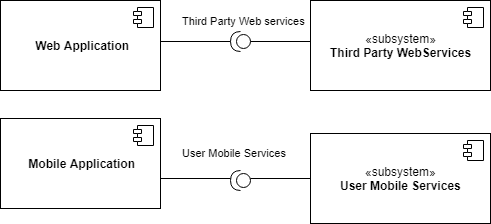
\includegraphics[scale=0.4]{DD/Pictures/component.png}
    \caption{Component view of \emph{TrackMe} System}
\end{figure}

\subsection{Component view of the Third Party Web Services}
\begin{figure}[H]
    \centering
    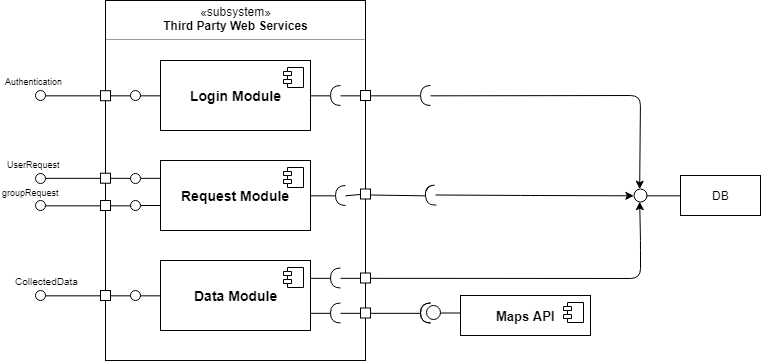
\includegraphics[scale=0.4]{DD/Pictures/ThirdPartyServiceDiagram(1).png}
    \caption{Third Party Web Service component}
    

\begin{itemize}
\item  The \underline{Login Module} manage the operations of authentication, allowing to the Third Party to be recognized and thus use the services of the System. It interacts with the database to check the credentials and retrieve the account information.

    \item The \underline{Request Module} is responsible of
    the requests dispatching: it offers to the Third Party the interfaces to fill out the forms to perform a user or a group request, and  forward them to the database. Among its internal function, it sends a notification to the target user when he/she is the subject of an user request to notify the event, and it performs the check security in case of group request, allowing the group requests only if the matched collected data belong to at least to 1000 individuals.
    
    \item The \underline{Data Module}  offers to the Third Parties all the functionalities to manage the performed requests, grouped by status (pending, accepted and refused), allows the consulting of the results, and calculates useful statistics on collected data. In case of subscription requests, it is its responsibility to update the Third party with the new data available with the frequency desired. It retrieves the selected data querying the database, that stores all the user records.
    This module is connected to Maps API to allow the consulting of user location data on an interactive map.
    
    
   \end{itemize} 
   
    
\end{figure}
\subsection{Component view of the User Mobile Service}

\begin{figure}[H]
    \centering
    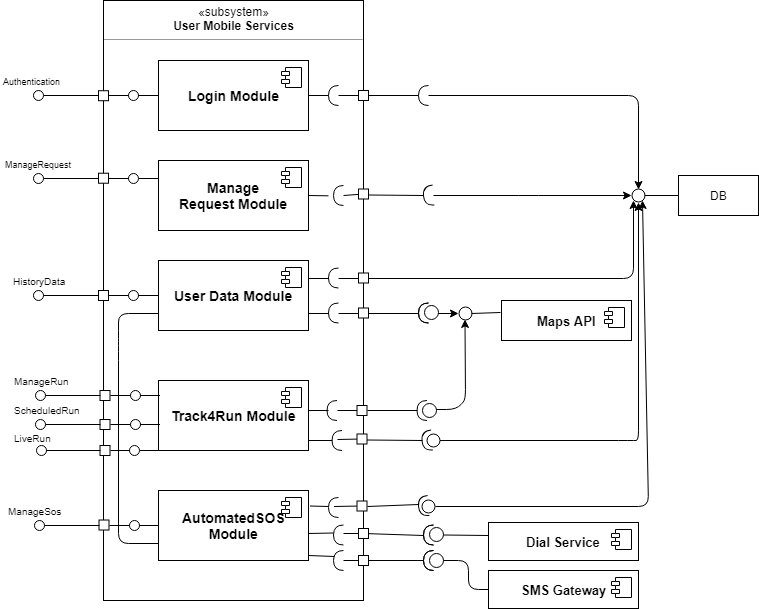
\includegraphics[scale=0.4]{DD/Pictures/UserServicesDiagram.png}
    \caption{User Mobile Services component }
\end{figure}

\begin{itemize}
    \item The \underline{Login Module}  manage the operations of authentication, allowing to the User to be recognized and thus use the services of the System. It interacts with the database to check the credentials and retrieve the account information.
    
    
    \item The \underline{Manage Request Module} offers to the user the functionalities to manage the incoming requests, providing all the information about the requested data. It interacts with the database, dispatching the user reply and notifies the sender Third Party about the occurred response.
    
    
    
    \item The \underline{User History Module} sends the new user's health and location data as soon as they have been collected by the smartwatch device  to the system database, that stores the records.
    
    It offers the interface to allow the User to visualize his/her History Data stored in the database, querying it with the time and location setting selected by the user, or performing a manual research. It is connected to the Maps API module to allow the visualization of user location data on an interactive map.
    
    
    \item The \underline{Track4Run Module} works as Run manager for the Track4Run system: it offers to the user the interfaces that allow to create and enroll to a run, visualize the list of the planned runs and follow live runs. It interacts with the Maps API module to manage the location data, and with the database to store new created runs and retrieved all the details about the runs. 
    
    \item The \underline{AutomatedSOS module} provides the functionalities concerning the AutomatedSOS system: it offers to the user the interface to enable or disable the service, to manage the emergency contact list and the emergency text message.
    
    It deals with all the tasks related to an emergency: it performs the checks on the health status and launches  an emergency state if it detects some anomalies in the health parameters. It interacts with the dial service to connect to the NHS, sending all the information related to the emergency, and with the SMS gateway, to notify the user's contact list with a text message.
    
    
    
\end{itemize}